% Created 2012-10-23 Tue 21:48
\documentclass[a4paper]{article}
\usepackage[utf8]{inputenc}
\usepackage{hyperref}
\usepackage{graphicx}
\usepackage{longtable}
\usepackage{float}
\usepackage{pdfpages}
\providecommand{\alert}[1]{\textbf{#1}}

\title{ADA-NCEPH Data Access Procedure}
\author{Ivan Hanigan and Steven McEachern}
\date{\today}
\hypersetup{
  pdfkeywords={},
  pdfsubject={},
  pdfcreator={Emacs Org-mode version 7.8.11}}

\begin{document}

\maketitle

% Org-mode is exporting headings to 3 levels.
\tableofcontents

\section{Introduction}
\label{sec-1}

The aim of this document is to describe the procedure for accessing restricted health data through the proposed ANU Secure Data Hub, administered by the ADA and NCEPH.

The following descibes procedures and processes for three different agents in the system, with different roles:
\begin{itemize}
\item Users,
\item User Administrators, and
\item Data Administrators.
\end{itemize}

The User and Data information that is used to control the actions of the system are stored in a Database at ANU referred to as the ANU-User-DB.
\newpage
\section{Getting Access}
\label{sec-2}

The ``Getting Access'' procedure to help users apply for and gain access to mortality data is shown in Figure 1, and a more detailed description of the process is shown in the Appendix, Figure 4. The process is a set of formally defined steps that are designed to move the User through two general stages:
\begin{itemize}
\item Requesting data: guiding the researcher through the process of (a) gaining Ethics Approval from a Human Research Ethics Committee, and (b) Project Level Approval from the Registrar of Births, Deaths and Marriages.
\item Providing data: provision of a confidentialised (often aggregated) dataset in an appropriately secured manner such as access to remote secure servers or encrypted archives accessed on local disk media, with security determined by (a) the nature of the data and (b) any project management related criteria.
\end{itemize}

\begin{figure}[!h]
\centering
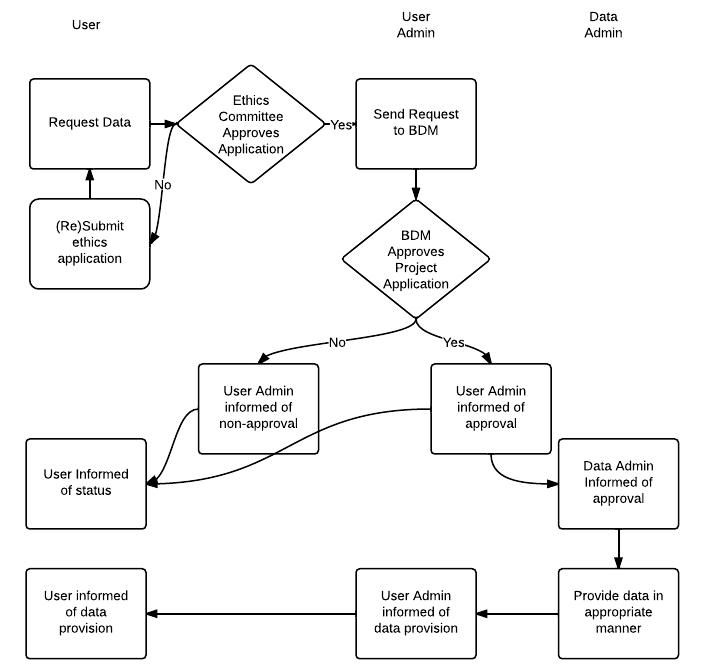
\includegraphics[width=1\textwidth]{DataAccessFlowDiagram-GettingAccess-general.png}
\caption{Flow Diagram of Getting Access}
\label{fig:DataAccessFlowDiagram-GettingAccess}
\end{figure}
\clearpage
\section{Managing Access}
\label{sec-3}

Procedures for managing access are shown in Figure 2 (and in the Appendix, Figure 5). These activities are intended to maintain information on the current state of projects using the mortality data, and to report any changes in situation to the State Registries. The User Administrator is responsible for conduct of the ``Managing Access'' procedures.

The process is initiated by running a query on the ANU-User-DB to make a list of all Projects and Users, and then each Project is sent a reminder to report any changes in Project Status (sent annually to coincide with a similar reminder sent by the ANU Human Research Ethics Committee). The purpose of these reminders is to ensure that Project management plans continue to consider data security as a primary concern, even during long multi-year projects where many project management and staffing issues inevitably arise.

Once a response is received, the User Administrator then enters the relevant information into the ANU-User-DB, and if the project has been concluded will then iniitate the final ``Ending Access'' process.
\section{Ending Access}
\label{sec-4}

The procedure for ending access aims to ensure that data are both securely and sustainably stored.  It is very important that files used for authorised projects are never re-used in un-authorised projects, but that future researchers may have the opportunity to create an authorised project and potentially replicate historical analyses.  This is an important part of reproducible research and the robust practice of scientific enquiry.
\subsection{Flow Chart for Ending Access}
\label{sec-4-1}
\subsubsection{\textbf{TODO} change this to the lucidchart version}
\label{sec-4-1-1}


\begin{figure}[!h]
\centering
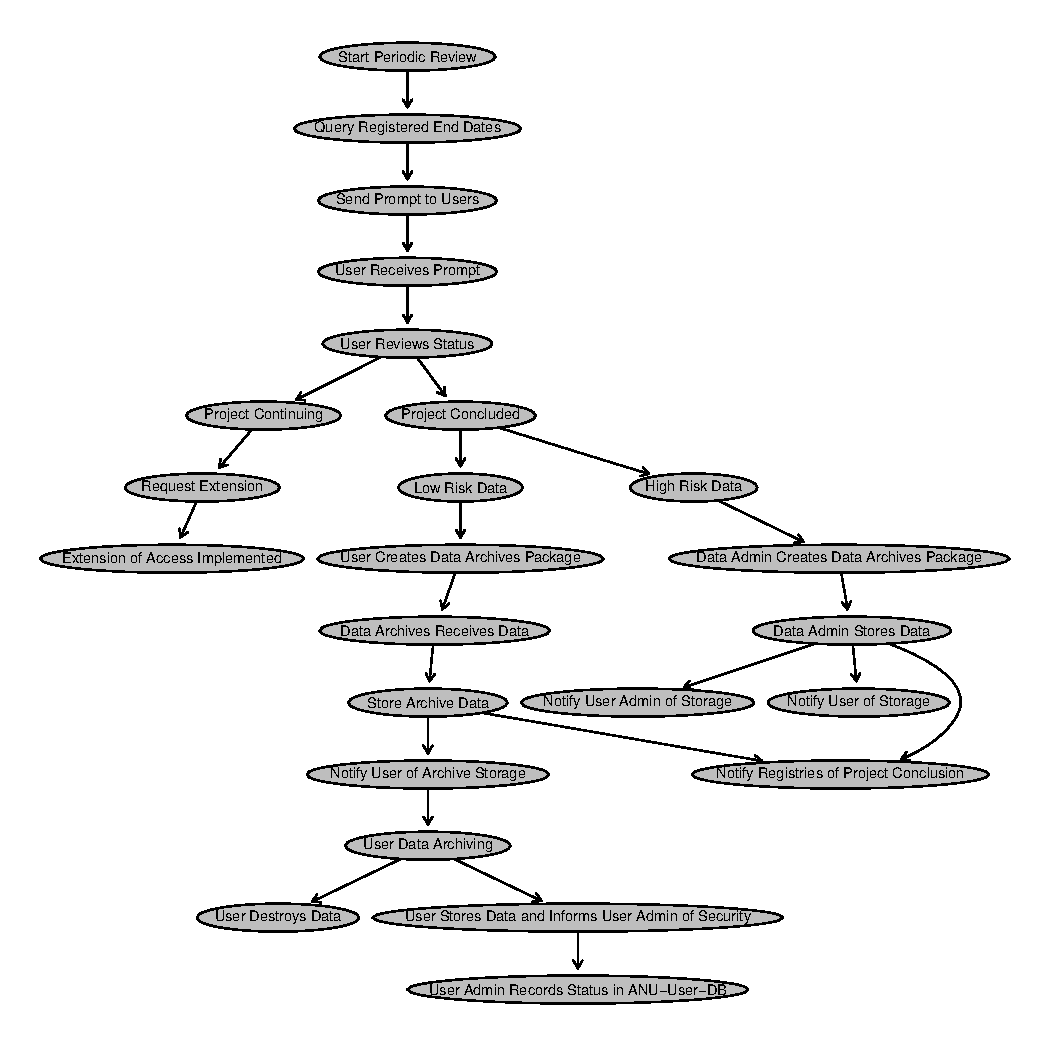
\includegraphics[width=\textwidth]{DataAccessFlowDiagram-EndAccess.pdf}
\caption{Flow Diagram for Ending Access}
\label{fig:DataAccessFlowDiagram-EndAccess}
\end{figure}
\clearpage
\section{Appendices}
\label{sec-5}
\subsection{Details of Steps for Getting Access}
\label{sec-5-1}

\begin{figure}[!h]
\centering
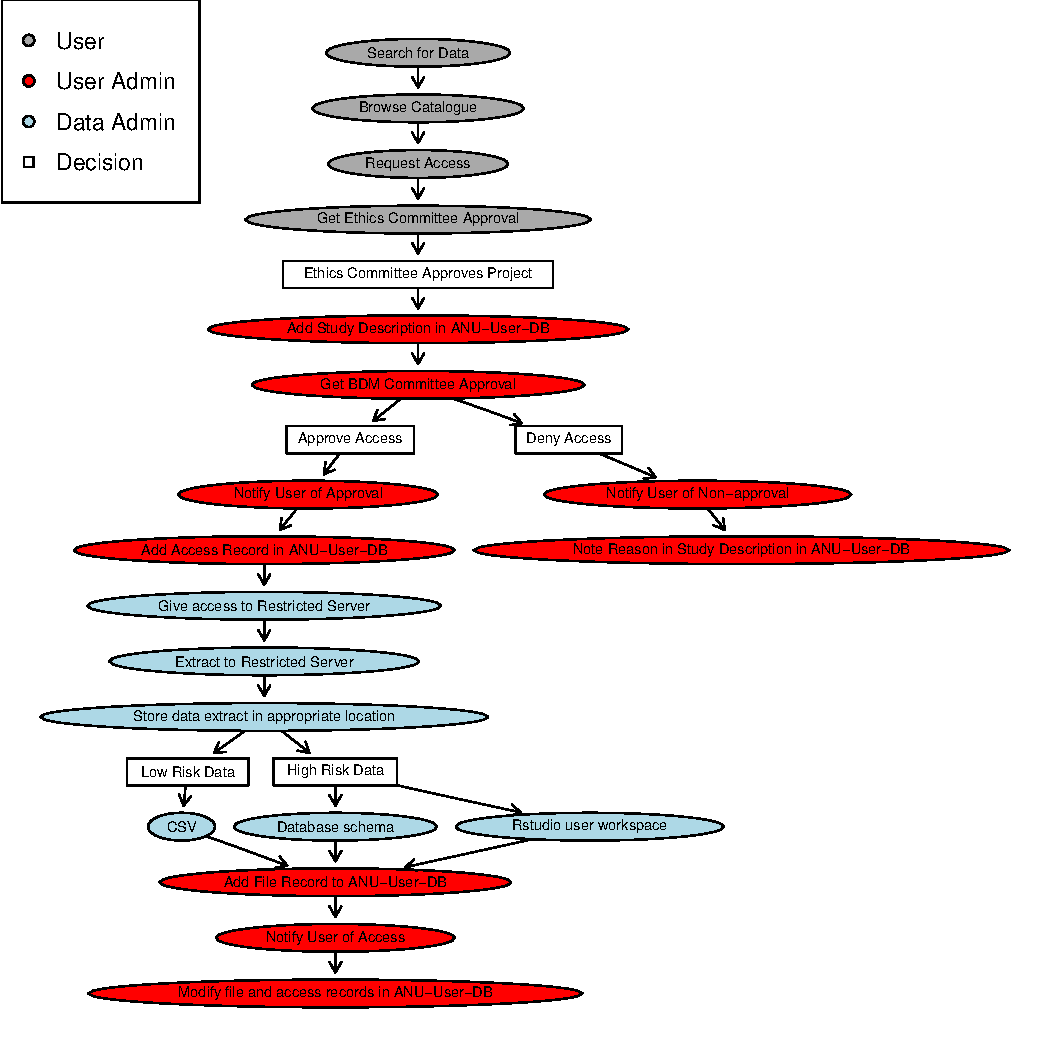
\includegraphics[width=1.4\textwidth]{DataAccessFlowDiagram-GettingAccess.pdf}
\caption{Detailed Flow Diagram of Getting Access}
\label{fig:DataAccessFlowDiagram-GettingAccess}
\end{figure}
\clearpage
\subsection{Details of Steps to Manage Access}
\label{sec-5-2}


\begin{figure}[!h]
\centering
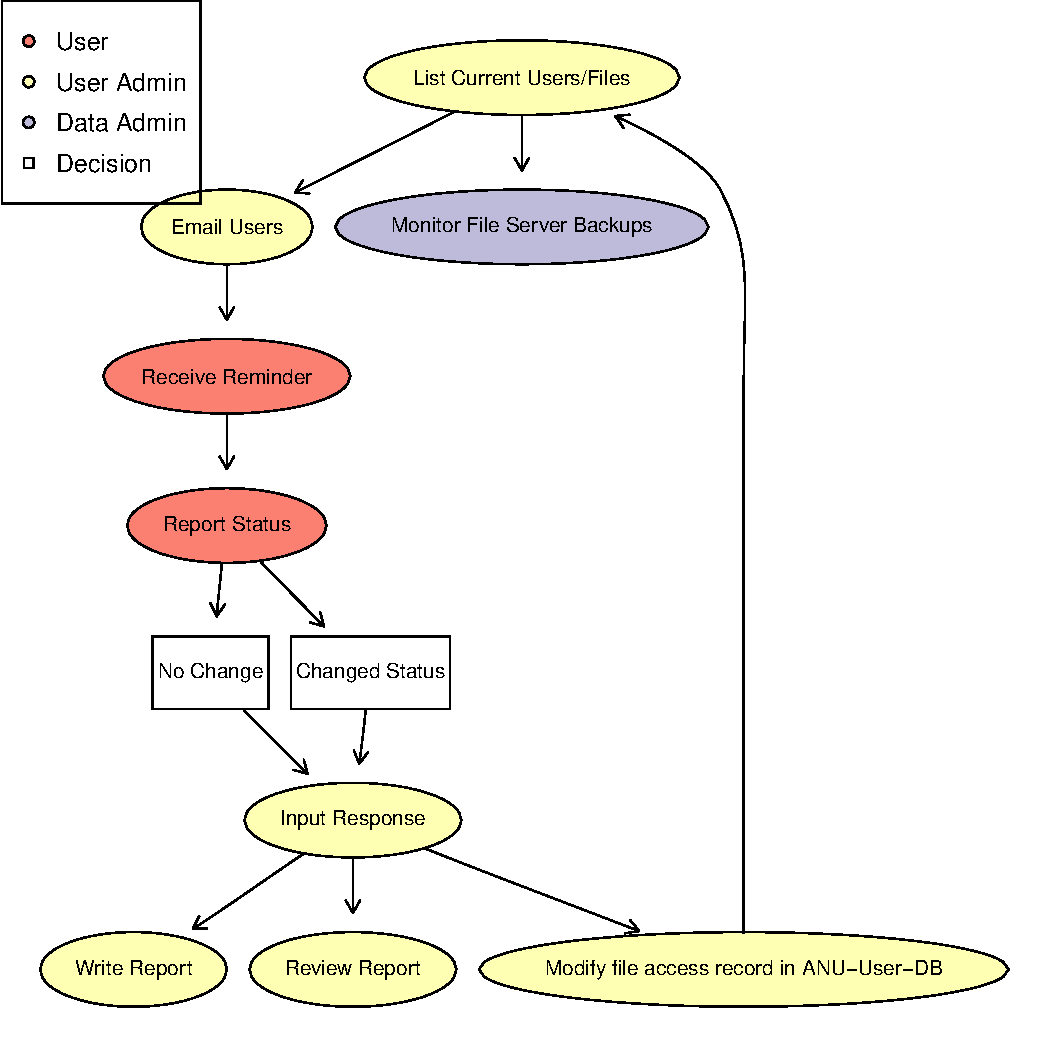
\includegraphics[width=1.4\textwidth]{DataAccessFlowDiagram-ManagingAccess.pdf}
\caption{Flow Diagram of Managing Access}
\label{fig:DataAccessFlowDiagram-ManagingAccess}
\end{figure}
\clearpage

\end{document}